\documentclass[a4paper,11pt]{article}

\usepackage[T1]{fontenc}
\usepackage[utf8]{inputenc}
\usepackage[english]{babel}
\usepackage{lmodern}
\usepackage{geometry}
\usepackage{hyperref}
\usepackage{xcolor}
\usepackage{tikz}
\usetikzlibrary{arrows.meta,positioning,fit,shapes.geometric,shapes.misc,calc,backgrounds}
\geometry{margin=2.2cm}

\hypersetup{
  colorlinks=true,
  linkcolor=blue!50!black,
  urlcolor=blue!50!black,
  pdftitle={ai4X Architecture},
  pdfauthor={nemron}
}

\title{ai4X Architecture}
\author{nemron}
\date{2026-02-21}

\tikzset{
  box/.style={draw, rounded corners, align=center, minimum width=3.2cm, minimum height=1cm, fill=blue!6},
  repo/.style={draw, rounded corners, align=left, minimum width=4.6cm, minimum height=1.0cm, fill=green!6},
  ext/.style={draw, rounded corners, align=center, minimum width=3.2cm, minimum height=1cm, fill=orange!10},
  flow/.style={draw, rounded corners, align=center, minimum width=3.1cm, minimum height=0.9cm, fill=purple!8},
  arrow/.style={-Latex, thick},
  linkarrow/.style={-Latex, thick, dashed}
}

\begin{document}
\maketitle

\section{Introduction}
This document explains the target architecture of the ai4X system in a deliberately gentle order.
We start with an overview and then zoom step by step into context, operations, components, flow, and directory structure.

\section{Handwritten Pre-Draft (External)}
As a conceptual pre-draft, a hand sketch exists at:
\texttt{/absolute/path/to/ai4X Initial Structure.jpeg}

The diagrams in this document are the formalized and consolidated version of that pre-draft.

\section{ai4X Overview (High-Level)}
\begin{center}
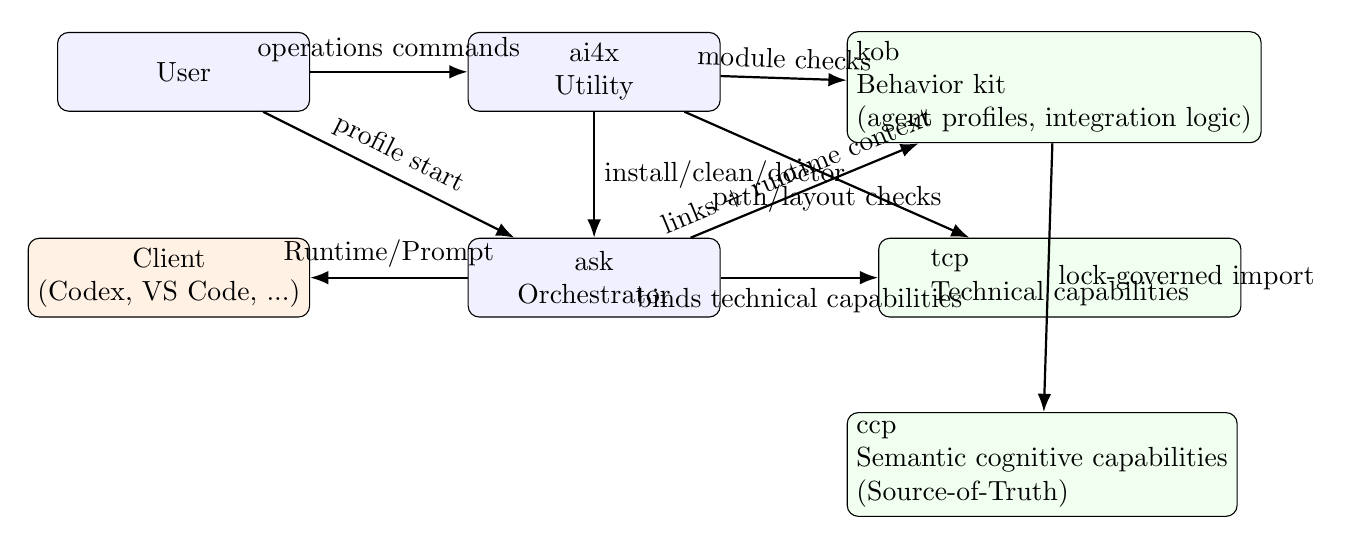
\begin{tikzpicture}[node distance=1.6cm and 2.0cm]
  \node[box] (user) {User};
  \node[box, right=of user] (ai4x) {ai4x\\Utility};
  \node[box, below=of ai4x] (ask) {ask\\Orchestrator};
  \node[repo, above right=1.2cm and 1.6cm of ask] (kob) {kob\\Behavior kit\\(agent profiles, integration logic)};
  \node[repo, right=of ask] (skills) {tcp\\Technical capabilities};
  \node[repo, below right=1.2cm and 1.6cm of ask] (rules) {ccp\\Semantic cognitive capabilities\\(Source-of-Truth)};
  \node[ext, left=of ask] (client) {Client\\(Codex, VS Code, ...)};

  \draw[arrow] (user) -- node[above]{operations commands} (ai4x);
  \draw[arrow] (user) -- node[above, sloped]{profile start} (ask);
  \draw[arrow] (ai4x) -- node[right]{install/clean/doctor} (ask);
  \draw[arrow] (ai4x) -- node[above, sloped]{module checks} (kob);
  \draw[arrow] (ai4x) -- node[below]{path/layout checks} (skills);
  \draw[arrow] (ask) -- node[above]{Runtime/Prompt} (client);
  \draw[arrow] (ask) -- node[above, sloped]{links + runtime context} (kob);
  \draw[arrow] (ask) -- node[below]{binds technical capabilities} (skills);
  \draw[arrow] (kob) -- node[right]{lock-governed import} (rules);
\end{tikzpicture}
\end{center}

\noindent
This view expresses the core idea on two layers:
\texttt{ai4x} orchestrates operations (install, clean, doctor), while \texttt{ask} orchestrates runtime.
\texttt{ask} remains technically neutral and connects user intent, client runtime, behavior, and capability sources at session time.
\texttt{kob} curates cognitive capabilities, \texttt{ccp} provides reusable rule modules,
and \texttt{tcp} provides technical capabilities.

\section{Context Diagram}
\begin{center}
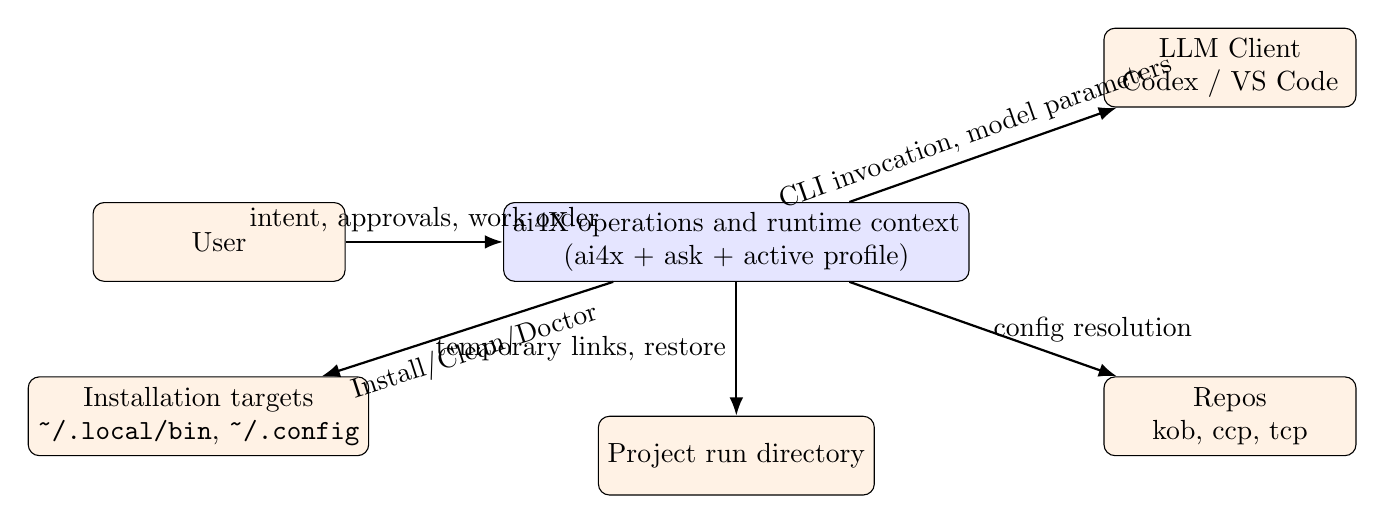
\begin{tikzpicture}[node distance=1.7cm and 2.0cm]
  \node[ext] (u) {User};
  \node[box, right=of u, minimum width=4.6cm, fill=blue!10] (sys) {ai4X operations and runtime context\\(ai4x + ask + active profile)};
  \node[ext, above right=1.2cm and 1.7cm of sys] (provider) {LLM Client\\Codex / VS Code};
  \node[ext, below right=1.2cm and 1.7cm of sys] (repos) {Repos\\kob, ccp, tcp};
  \node[ext, below=of sys] (run) {Project run directory};
  \node[ext, below left=1.2cm and 1.7cm of sys] (targets) {Installation targets\\\texttt{\textasciitilde/.local/bin}, \texttt{\textasciitilde/.config}};

  \draw[arrow] (u) -- node[above]{intent, approvals, work order} (sys);
  \draw[arrow] (sys) -- node[above, sloped]{CLI invocation, model parameters} (provider);
  \draw[arrow] (sys) -- node[right]{config resolution} (repos);
  \draw[arrow] (sys) -- node[left]{temporary links, restore} (run);
  \draw[arrow] (sys) -- node[below, sloped]{Install/Clean/Doctor} (targets);
\end{tikzpicture}
\end{center}

\noindent
The context diagram clearly separates system boundary and external world:
ai4X handles operations and lifecycle control while domain content and rules
reside in separate repositories.
This keeps behavior/rule changes decoupled from the runtime launcher.

\section{Operations Diagram (\texttt{ai4x} Utility)}
\begin{center}
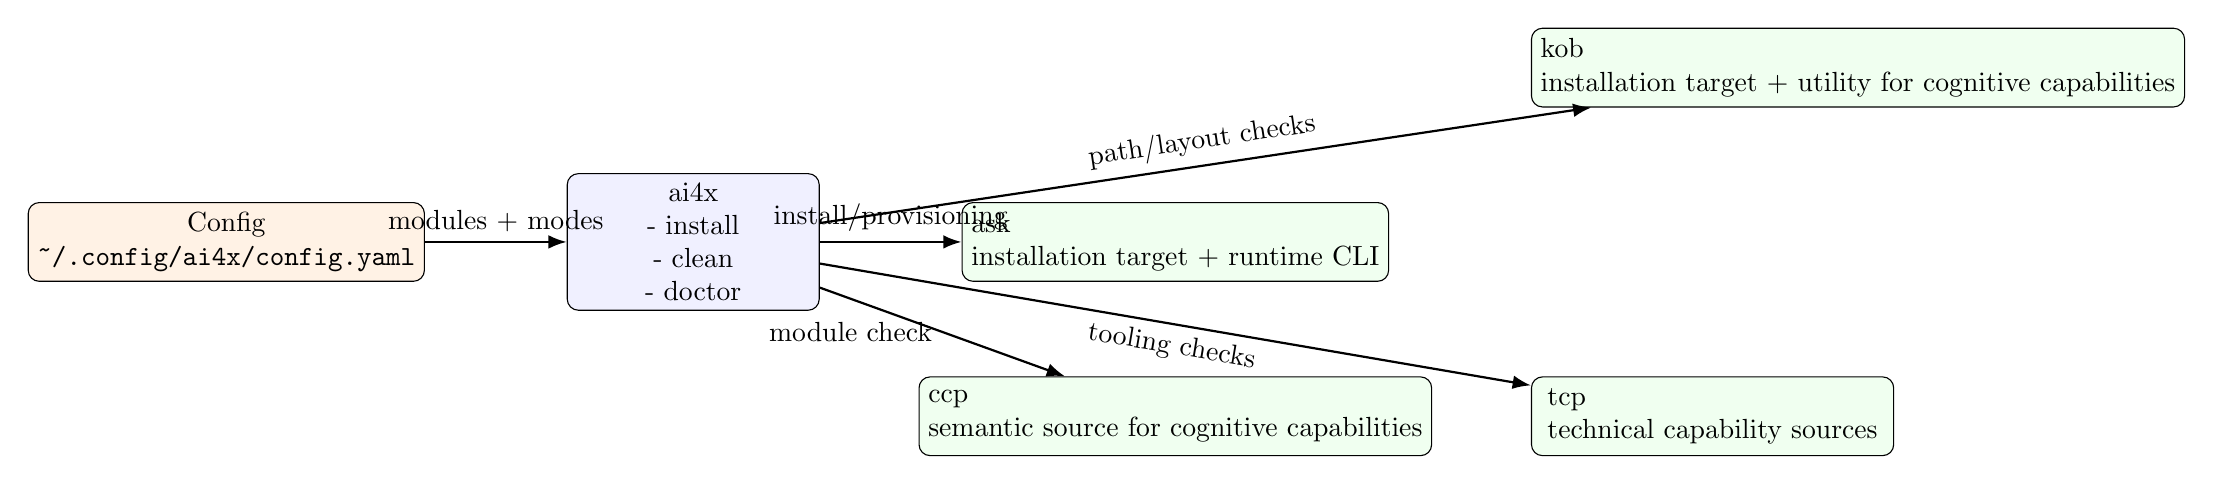
\begin{tikzpicture}[node distance=1.2cm and 1.8cm]
  \node[box] (ai4x) {ai4x\\- install\\- clean\\- doctor};
  \node[repo, right=of ai4x] (ask) {ask\\installation target + runtime CLI};
  \node[repo, above right=1.2cm and 1.8cm of ask] (kob) {kob\\installation target + utility for cognitive capabilities};
  \node[repo, below right=1.2cm and 1.8cm of ask] (skills) {tcp\\technical capability sources};
  \node[repo, below=of ask] (rules) {ccp\\semantic source for cognitive capabilities};
  \node[ext, left=of ai4x] (cfg) {Config\\\texttt{\textasciitilde/.config/ai4x/config.yaml}};

  \draw[arrow] (cfg) -- node[above]{modules + modes} (ai4x);
  \draw[arrow] (ai4x) -- node[above]{install/provisioning} (ask);
  \draw[arrow] (ai4x) -- node[above, sloped]{path/layout checks} (kob);
  \draw[arrow] (ai4x) -- node[left]{module check} (rules);
  \draw[arrow] (ai4x) -- node[below, sloped]{tooling checks} (skills);
\end{tikzpicture}
\end{center}

\noindent
This diagram isolates the operations layer:
\texttt{ai4x} reads module configuration, executes install/cleanup,
and validates integration state via \texttt{doctor}.
Session orchestration is intentionally delegated to \texttt{ask}.

\section{Component Diagram}
\begin{center}
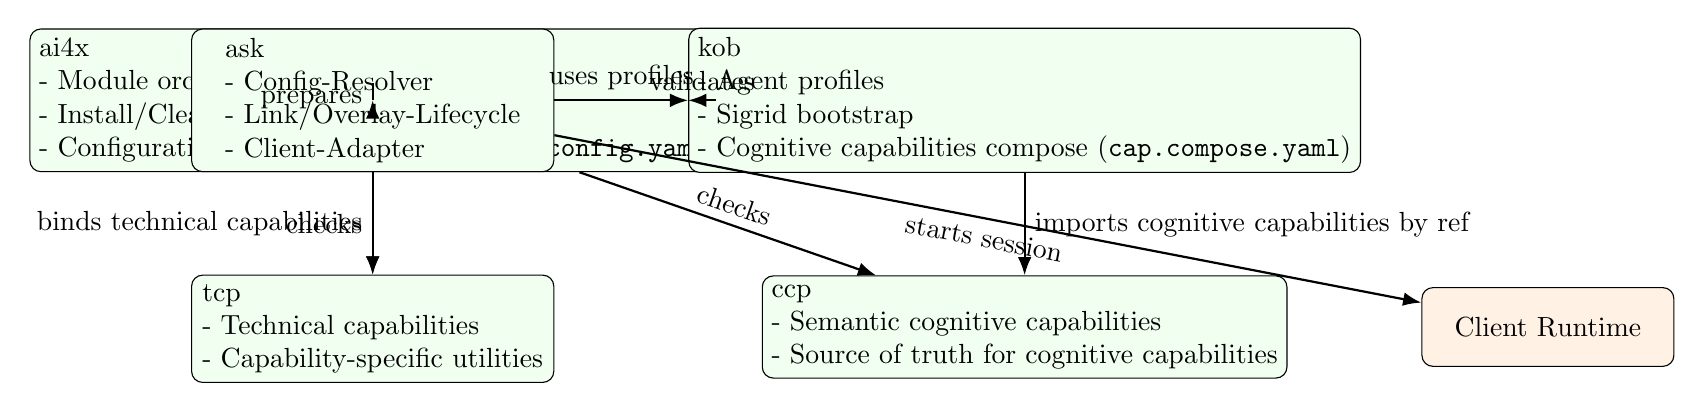
\begin{tikzpicture}[node distance=1.3cm and 1.7cm]
  \node[repo] (ai4x) {ai4x\\- Module orchestration\\- Install/Clean/Doctor\\- Configuration source: \texttt{\textasciitilde/.config/ai4x/config.yaml}};
  \node[repo] (ask) {ask\\- Config-Resolver\\- Link/Overlay-Lifecycle\\- Client-Adapter};
  \node[repo, right=of ask] (kob) {kob\\- Agent profiles\\- Sigrid bootstrap\\- Cognitive capabilities compose (\texttt{cap.compose.yaml})};
  \node[repo, below=of kob] (rules) {ccp\\- Semantic cognitive capabilities\\- Source of truth for cognitive capabilities};
  \node[repo, below=of ask] (skills) {tcp\\- Technical capabilities\\- Capability-specific utilities};
  \node[ext, right=of rules] (client) {Client Runtime};

  \draw[arrow] (ai4x) -- node[left]{prepares} (ask);
  \draw[arrow] (ai4x) -- node[above, sloped]{validates} (kob);
  \draw[arrow] (ai4x) -- node[above, sloped]{checks} (rules);
  \draw[arrow] (ai4x) -- node[left]{checks} (skills);
  \draw[arrow] (ask) -- node[above]{uses profiles} (kob);
  \draw[arrow] (ask) -- node[left]{binds technical capabilities} (skills);
  \draw[arrow] (kob) -- node[right]{imports cognitive capabilities by ref} (rules);
  \draw[arrow] (ask) -- node[below, sloped]{starts session} (client);
\end{tikzpicture}
\end{center}

\noindent
The components are modular with clear responsibilities:
\texttt{ai4x} orchestrates operations, \texttt{ask} orchestrates runtime, \texttt{kob} defines behavior,
\texttt{ccp} provides cognitive-capability content, and \texttt{tcp} provides technical capabilities.
This separation improves maintainability, testable contracts, and release readiness.

\section{Flow Diagram (Operations + Sigrid)}
\begin{center}
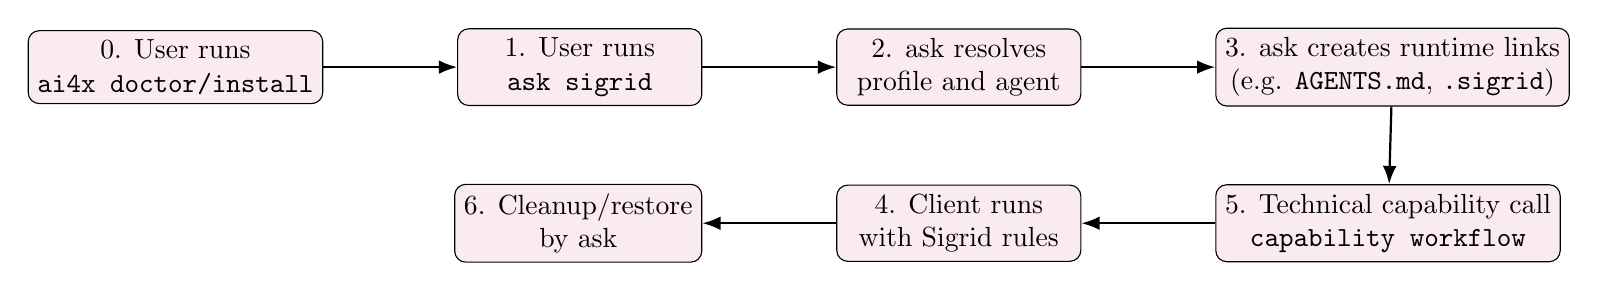
\begin{tikzpicture}[node distance=1.0cm and 1.7cm]
  \node[flow] (f0) {0. User runs\\\texttt{ai4x doctor/install}};
  \node[flow, right=of f0] (f1) {1. User runs\\\texttt{ask sigrid}};
  \node[flow, right=of f1] (f2) {2. ask resolves\\profile and agent};
  \node[flow, right=of f2] (f3) {3. ask creates runtime links\\(e.g. \texttt{AGENTS.md}, \texttt{.sigrid})};
  \node[flow, below=of f2] (f4) {4. Client runs\\with Sigrid rules};
  \node[flow, right=of f4] (f5) {5. Technical capability call\\\texttt{capability workflow}};
  \node[flow, left=of f4] (f6) {6. Cleanup/restore\\by ask};

  \draw[arrow] (f0) -- (f1);
  \draw[arrow] (f1) -- (f2);
  \draw[arrow] (f2) -- (f3);
  \draw[arrow] (f3) -- (f5);
  \draw[arrow] (f5) -- (f4);
  \draw[arrow] (f4) -- (f6);
\end{tikzpicture}
\end{center}

\noindent
The flow deliberately separates operations and runtime phases:
before session start, \texttt{ai4x} validates a consistent integration state.
Configuration and linking then happen in \texttt{ask} before client startup,
domain work happens inside the session,
and \texttt{ask} restores the initial state after the session.
This keeps runs reproducible and non-destructive.

\section{Runtime overlay for \texttt{CODEX\_HOME} (technical view)}
\begin{center}
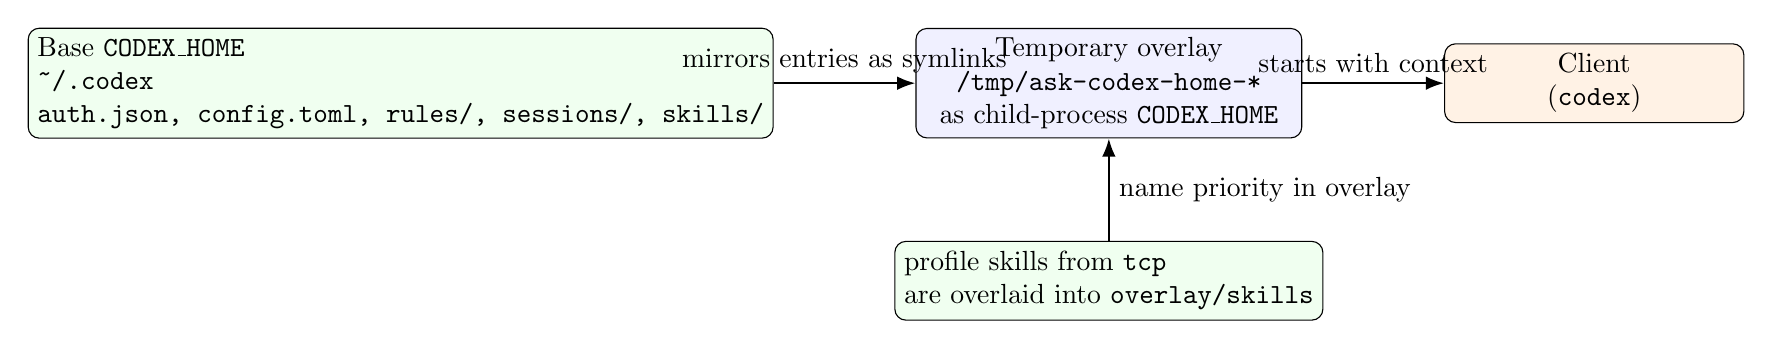
\begin{tikzpicture}[node distance=1.3cm and 1.8cm]
  \node[repo, minimum width=4.9cm] (base) {Base \texttt{CODEX\_HOME}\\\texttt{\textasciitilde/.codex}\\\texttt{auth.json, config.toml, rules/, sessions/, skills/}};
  \node[box, right=of base, minimum width=4.9cm] (overlay) {Temporary overlay\\\texttt{/tmp/ask-codex-home-*}\\as child-process \texttt{CODEX\_HOME}};
  \node[ext, right=of overlay, minimum width=3.8cm] (client) {Client\\(\texttt{codex})};
  \node[repo, below=of overlay, minimum width=5.2cm] (skills) {profile skills from \texttt{tcp}\\are overlaid into \texttt{overlay/skills}};

  \draw[arrow] (base) -- node[above]{mirrors entries as symlinks} (overlay);
  \draw[arrow] (overlay) -- node[above]{starts with context} (client);
  \draw[arrow] (skills) -- node[right]{name priority in overlay} (overlay);
\end{tikzpicture}
\end{center}

\noindent
The overlay mechanism has four explicit steps:
\begin{enumerate}
  \item Determine the base directory: \texttt{CODEX\_HOME}, or fallback to \texttt{\textasciitilde/.codex}.
  \item Create an overlay directory and set it as \texttt{CODEX\_HOME} only for the started client process.
  \item mirror all base entries except \texttt{skills/} as symlinks, then
        build \texttt{overlay/skills/} from base skills plus profile skills.
  \item Remove overlay and runtime links after session end.
\end{enumerate}

\noindent
Important for user trust:
\begin{itemize}
  \item \texttt{auth.json} and \texttt{config.toml} stay effective.
  \item If no auth file exists in base \texttt{CODEX\_HOME}, the normal client login flow appears.
  \item \texttt{rules/} and existing \texttt{sessions/} remain visible and usable.
  \item With existing \texttt{sessions/}, \texttt{ask} runs remain resumable in the normal session store.
  \item When skill names collide, only the profile skill in the overlay is active; base \texttt{skills/} remains unchanged.
  \item Scope is process-local: \texttt{ask} sets \texttt{CODEX\_HOME} for the child process, not globally.
\end{itemize}

\section{Directory structure including symbolic links (illustrative)}
\begin{center}
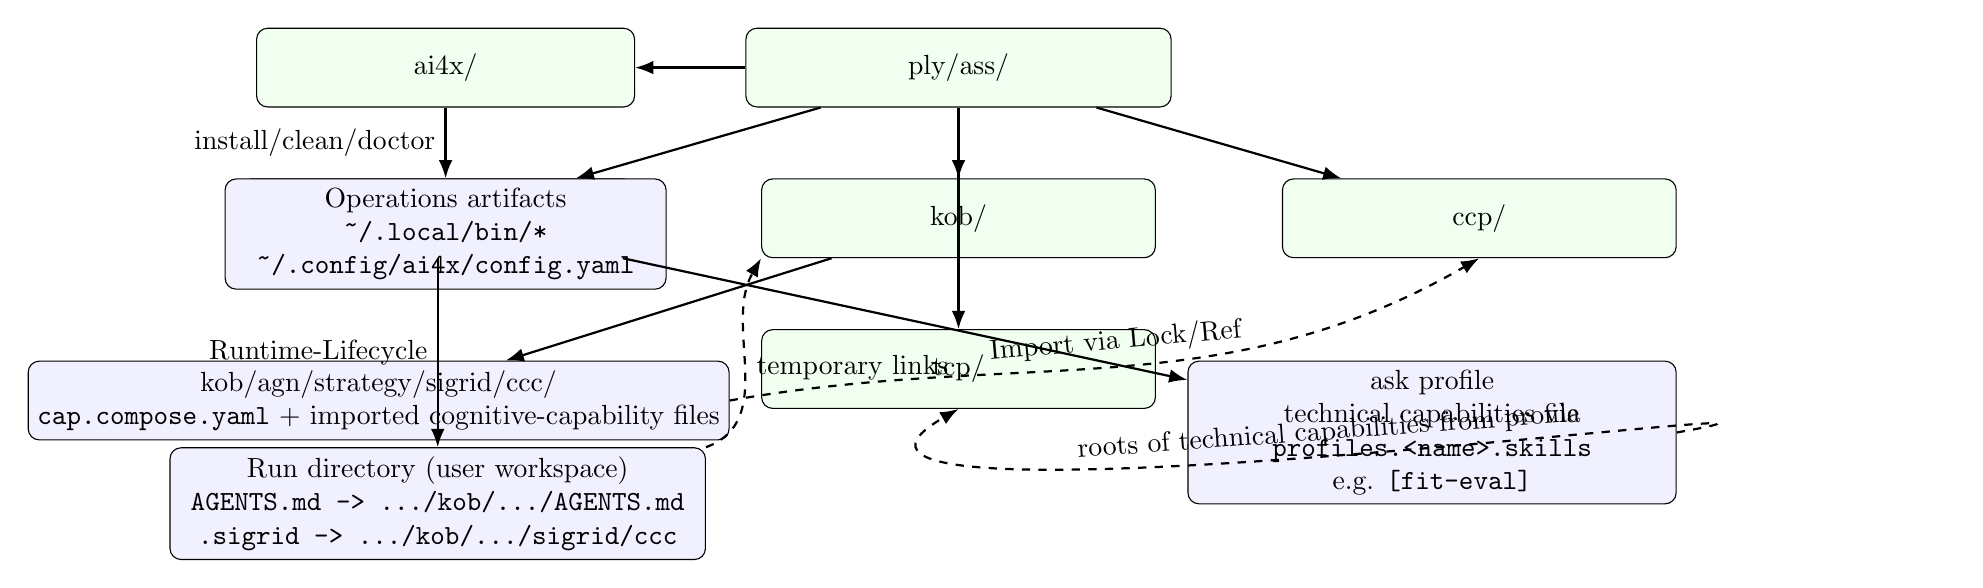
\begin{tikzpicture}[node distance=0.9cm and 1.4cm]
  \node[repo, minimum width=5.4cm] (root) {ply/ass/};
  \node[repo, left=of root, minimum width=4.8cm] (ai4xrepo) {ai4x/};
  \node[repo, below left=of root, minimum width=5.0cm] (askrepo) {ask/};
  \node[repo, below=of root, minimum width=5.0cm] (kobrepo) {kob/};
  \node[repo, below right=of root, minimum width=5.0cm] (rulesrepo) {ccp/};
  \node[repo, below=of kobrepo, minimum width=5.0cm] (skillsrepo) {tcp/};
  \node[box, below=of ai4xrepo, minimum width=5.6cm] (ops) {Operations artifacts\\\texttt{\textasciitilde/.local/bin/*}\\\texttt{\textasciitilde/.config/ai4x/config.yaml}};

  \node[box, below left=1.3cm and 0.4cm of kobrepo, minimum width=6.2cm] (kobrules) {kob/agn/strategy/sigrid/ccc/\\\texttt{cap.compose.yaml} + imported cognitive-capability files};
  \node[box, below right=1.3cm and 0.4cm of kobrepo, minimum width=6.2cm] (askskills) {ask profile\\technical capabilities via\\\texttt{profiles.<name>.skills}\\e.g. \texttt{[fit-eval]}};

  \node[box, below=2.4cm of askrepo, minimum width=6.8cm] (run) {Run directory (user workspace)\\\texttt{AGENTS.md -> .../kob/.../AGENTS.md}\\\texttt{.sigrid -> .../kob/.../sigrid/ccc}};

  \draw[arrow] (root) -- (askrepo);
  \draw[arrow] (root) -- (kobrepo);
  \draw[arrow] (root) -- (rulesrepo);
  \draw[arrow] (root) -- (skillsrepo);
  \draw[arrow] (root) -- (ai4xrepo);
  \draw[arrow] (ai4xrepo) -- node[left]{install/clean/doctor} (ops);

  \draw[arrow] (kobrepo) -- (kobrules);
  \draw[linkarrow] (kobrules.east) to[out=10,in=-150] node[above, sloped]{Import via Lock/Ref} (rulesrepo.south);

  \draw[arrow] (askrepo) -- (askskills);
  \draw[linkarrow] (askskills.east) to[out=10,in=-150] node[above, sloped]{roots of technical capabilities from profile} (skillsrepo.south);

  \draw[arrow] (askrepo.south) -- node[left]{Runtime-Lifecycle} (run.north);
  \draw[linkarrow] (run.north east) to[out=20,in=-120] node[right]{temporary links} (kobrepo.south west);
\end{tikzpicture}
\end{center}

\noindent
The structure diagram combines repository view and runtime view:
\texttt{ai4x} manages operations artifacts,
cognitive capabilities are reproducibly imported from \texttt{ccp},
technical capabilities are referenced from \texttt{tcp},
and \texttt{ask} creates temporary runtime links in the working directory.
This clarifies which relations are persistent (repository level)
and which are runtime-only.

\section{Conclusion and release-candidate perspective}
With the current structure (separate repos, lock-governed cognitive capability integration, clear runtime lifecycle logic)
ai4X is architecturally RC-ready for broad user testing.
For production release, finalize CI gates, changelog automation, and the formal cross-repo release process.

\end{document}
